\documentclass{article}
\LARGE
% Language setting
% Replace `english' with e.g. `spanish' to change the document language
\usepackage[english]{babel}

% Set page size and margins
% Replace `letterpaper' with `a4paper' for UK/EU standard size
\usepackage[letterpaper,top=2cm,bottom=2cm,left=3cm,right=3cm,marginparwidth=1.75cm]{geometry}


\usepackage{tikz}
\usetikzlibrary{shapes.geometric, arrows}
\tikzstyle{startstop} = [rectangle, rounded corners, minimum width=3cm, minimum height=1cm,text centered, draw=black, fill=red!30]
\tikzstyle{io} = [trapezium, trapezium left angle=70, trapezium right angle=110, minimum width=3cm, minimum height=1cm, text centered, draw=black, fill=blue!30]
\tikzstyle{process} = [rectangle, minimum width=3cm, minimum height=1cm, text centered, draw=black, fill=orange!30]
\tikzstyle{decision} = [diamond, minimum width=3cm, minimum height=1cm, text centered, draw=black, fill=green!30]
\tikzstyle{arrow} = [thick,->,>=stealth]




\pgfdeclarelayer{bg}
\pgfsetlayers{bg,main}

% Useful packages
\usepackage{amsmath}
\usepackage{amsfonts}
\usepackage{graphicx}
\usepackage[colorlinks=true, allcolors=cyan]{hyperref}
\numberwithin{equation}{section}
\usepackage{graphicx,wrapfig,lipsum,subfigure,sidecap,epsfig}
\usepackage{caption}
\usepackage{cancel}
%\usepackage{graphicx,subfigure,sidecap,epsfig} % Rouslan's subfig package
\usepackage{soul}
%\usepackage[colorlinks=true,linkcolor=red]{hyperref}%
\usepackage{mathtools}
\usepackage{eqparbox}
\usepackage{float} % \figure{}[H] IN PLACE VIEW
\usepackage[capitalize]{cleveref} % smart references in one bracket
\usepackage{hyperref}
\usepackage{amssymb} % rightleft arrows
\usepackage{cancel} % \cancelto{<value>}{expression} diagonally
\usepackage[mathscr]{euscript}
\DeclareSymbolFont{rsfs}{U}{rsfs}{m}{n}
\DeclareSymbolFontAlphabet{\mathscrsfs}{rsfs}
\usepackage{MnSymbol}


%
% CREF rules
% Equation(s)
\crefformat{equation}{#2Eq. (#1)#3}
\crefrangeformat{equation}{#3Eqs. (#1)#4 to #5(#2)#6}
\crefmultiformat{equation}{#2Eqs. (#1)#3}{ and #2(#1)#3}{, #2(#1)#3}{ and #2(#1)#3}
\crefrangemultiformat{equation}{#3Eqs. ((#1))#4 to #5((#2))#6}{ and #3(#1)#4 to #5(#2)#6}{, #3(#1)#4 to #5(#2)#6}{ and #3(#1)#4 to #5(#2)#6}
% Plural eqn
\crefformat{pluralequation}{#2Eqs.~(#1)#3}
% System
\crefformat{system}{#2Sys.~(#1)#3}
\crefrangeformat{system}{#3Sys. (#1)#4 to #5(#2)#6}
\crefmultiformat{system}{#2Sys. (#1)#3}{ and #2(#1)#3}{, #2(#1)#3}{ and #2(#1)#3}
\crefrangemultiformat{system}{#3Sys. ((#1))#4 to #5((#2))#6}{ and #3(#1)#4 to #5(#2)#6}{, #3(#1)#4 to #5(#2)#6}{ and #3(#1)#4 to #5(#2)#6}
% Boundary conditions
\crefformat{bc}{#2BC (#1)#3}
\crefrangeformat{bc}{#3BCs (#1)#4 to #5(#2)#6}
\crefmultiformat{bc}{#2BCs (#1)#3}{ and #2(#1)#3}{, #2(#1)#3}{ and #2(#1)#3}
\crefrangemultiformat{bc}{#3BCs ((#1))#4 to #5((#2))#6}{ and #3(#1)#4 to #5(#2)#6}{, #3(#1)#4 to #5(#2)#6}{ and #3(#1)#4 to #5(#2)#6}
% Steps
\crefformat{step}{#2Step (#1)#3}
\crefrangeformat{step}{#3Steps (#1)#4 to #5(#2)#6}
\crefmultiformat{step}{#2Steps (#1)#3}{ and #2(#1)#3}{, #2(#1)#3}{ and #2(#1)#3}
\crefrangemultiformat{step}{#3Steps ((#1))#4 to #5((#2))#6}{ and #3(#1)#4 to #5(#2)#6}{, #3(#1)#4 to #5(#2)#6}{ and #3(#1)#4 to #5(#2)#6}
%diagram
\crefformat{diagram}{#2Diagram (#1)#3}
\crefrangeformat{diagram}{#3Diagrams (#1)#4 to #5(#2)#6}
\crefmultiformat{diagram}{#2Diagrams (#1)#3}{ and #2(#1)#3}{, #2(#1)#3}{ and #2(#1)#3}
\crefrangemultiformat{diagram}{#3Diagrams ((#1))#4 to #5((#2))#6}{ and #3(#1)#4 to #5(#2)#6}{, #3(#1)#4 to #5(#2)#6}{ and #3(#1)#4 to #5(#2)#6}
%algorithm
\crefformat{algorithm}{#2Algorithm (#1)#3}
\crefrangeformat{algorithm}{#3Algorithms (#1)#4 to #5(#2)#6}
\crefmultiformat{algorithm}{#2Algorithms (#1)#3}{ and #2(#1)#3}{, #2(#1)#3}{ and #2(#1)#3}
\crefrangemultiformat{algorithm}{#3Algorithms ((#1))#4 to #5((#2))#6}{ and #3(#1)#4 to #5(#2)#6}{, #3(#1)#4 to #5(#2)#6}{ and #3(#1)#4 to #5(#2)#6}



%\usepackage[sortcites=true]{biblatex} % biblatex DOEST WORK WITH LIVE TYPESETTER
\usepackage[nocompress]{cite}
%\bibliographystyle{ieeetr} % trash style mess up the order in bib

\graphicspath{{figures/}}


%%% Todos
\newcommand{\todo}[1]{\vspace{5 mm}\par \noindent
\marginpar{\textsc{\tiny \hspace{0.5cm} ToDo}} \framebox{\begin{minipage}[c]{0.95
\textwidth} \small \tt #1 \end{minipage}}\vspace{5 mm}\par}



\title{Discrete stream function method \\ for the incompressible Navier-Stokes equations \\with simple boundary conditions}
\author{Rauan}

\begin{document}
\maketitle

\begin{abstract}
The goal of these notes is to present the detailed overview of discrete stream function method for solving incompressible Navier-Stokes equations with simple boundary conditions. We will discuss in detail the scheme formulation, transient and spatial discretizations. Special attention will be paid to the change of unknown variables. After studying these notes one must get a coherent picture of the application of discrete stream function method to incompressible flows with simple Boundary Conditions (BCs) and be able to implement the scheme in code.
\end{abstract}

\tableofcontents

\section{Introduction}\label{sec:introduction}

In these notes we will be concerned with the discretization of the Navier-Stokes equations describing the flow of an incompressible fluid past the 2-dimensional cylinder with a singular boundary force f added to the momentum equation as a continuous analog of the immersed boundary formulation:
\begin{subequations}
\label[pluralequation]{eqs:NSE}
\begin{align}
\label{eqn:momentum-intro}
\frac{\partial \boldsymbol{v}}{\partial t} + \boldsymbol{v} \cdot \nabla \boldsymbol{v} &= -\nabla p + \epsilon \nabla \cdot \nabla \boldsymbol{v} +\int_{s}\boldsymbol{f}(\xi(s,t))\delta(\xi-x)ds\\
\label{eqn:continuity}
\nabla \cdot \boldsymbol{v} &= 0,\\
\boldsymbol{v}(\xi(s,t)) &= \int_x\boldsymbol{v}(x)\delta(x - \xi)dx = \boldsymbol{v}_B(\xi(x,t)),
\end{align}
\end{subequations}
which are written here in the non-dimensional form, i.e. $\epsilon \equiv Re^{-1}$ for brevity; also $\boldsymbol{v}$ is the velocity and $p$ pressure fields. The boundary conditions are assumed to be simple, i.e.  Dirichlet and Neumann for the normal and tangential velocities, respectively. Spatial variable $x$ represents position in the flow field, $\mathscrsfs{D}$, and $\xi$ denotes coordinates along the immersed boundary, $\partial \mathscrsfs{B}$ having a velocity of $\boldsymbol{v}_B$. The geometry of the immersed object $\mathscrsfs{B}$ is considered to be of arbitrary shape. 


\section{Discretization}\label{sec:discretization}

\begin{figure}[H] % here - h, bottom - b, top - t
  \centering{
  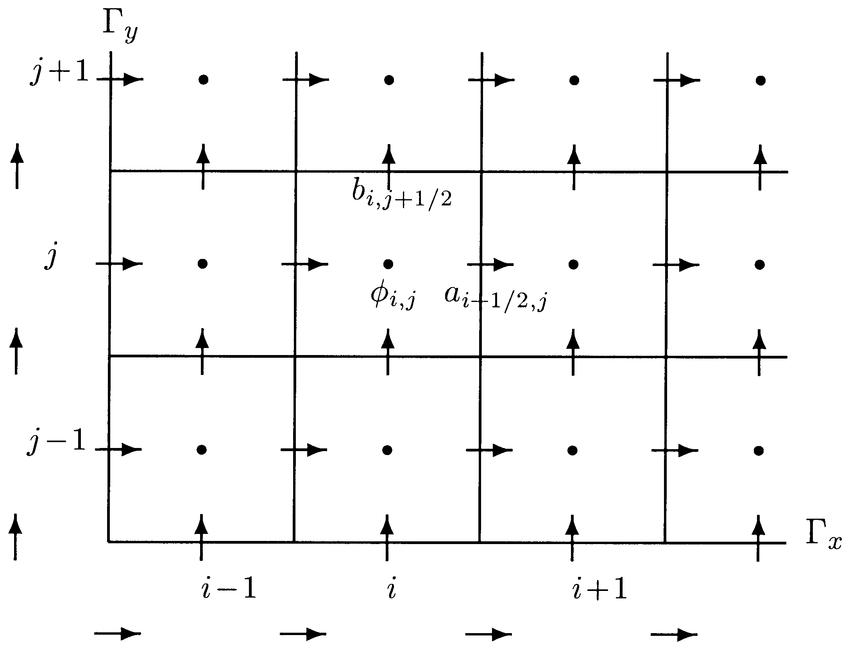
\includegraphics[width=0.55\paperwidth]{fig1}
  }
  \caption{Staggered grid discretization of a two-dimensional computational domain $\mathscrsfs{D}$ and immersed boundary formulation for a body $\mathscrsfs{B}$ depicted by a shaded object. The horizontal and vertical arrows ($\rightarrow$, $\uparrow$) represent the discrete $u_i$ and $v_i$ velocity components, respectively. Pressure $p_i$ is positioned at the center of each cell ($\times$). Lagrangian points, $\xi_k$ = ($\xi_k$, $\eta_k$), along $\partial\mathscrsfs{B}$ are shown with filled squares ($\filledsquare$) where boundary forces $\boldsymbol{f}_k=(f_{x,k},f_{y,k})$ are applied ($\Rightarrow,\Uparrow$).}\label{fig:1}
\end{figure}

The above system is discretized with a standard staggered Cartesian grid finite volume method. The mesh and variable locations are depicted in \cref{fig:1}. The computational domain, $\mathscrsfs{D}$, is represented by a Cartesian grid, ($x_i, y_i$), and the immersed boundary, $\mathscrsfs{B}$ is described by a set of Lagrangian points, ($\xi_k,\eta_k$), which can be a function of time.

We can rewrite \cref{eqs:NSE} using discrete differential operators as 
\begin{equation}\label[pluralequation]{eqs:discrete-nse}
\begin{aligned}
	M\frac{dq}{dt} + Gp - Hf &= \mathbf{N}(q) + Lq + bc_1&\text{ (momentum),}\\
	Dq &= 0 + bc_2&\text{ (continuity),}\\
	Eq & = \boldsymbol{v}_B^{n+1} &\text{ (no-slip condition),}
	\end{aligned}
\end{equation}
where $q=(  u\Delta y,v\Delta x )$, $p$ and $f$ are the discrete velocity flux vector, pressure, and boundary force. Discretized non-linear advective term $\boldsymbol{v}\cdot\nabla \boldsymbol{v}$ is denoted as $\mathbf{N}(q)$, whereas operators $M$, $L$ are mass matrix and discrete Laplacian respectively. Operators $G$ and $D$ are discrete gradient and divergence matrices s.t. $D=-G^T$ and \cite{Chang:2002,Perot:1993}. The rest operators $E$ and $H$ are the interpolation and regularization operators resulting from the regularization of the Dirac delta functions in momentum and no-slip equations, which are constructed in such a way that $E=-H^T$. No-slip constraint is enforced by equating the boundary velocity, $\boldsymbol{v}_B$, to the velocity value along $\partial \mathscrsfs{B}$ interpolated by $E$ from the neighbouring cells. Regularization operator diffuses the singular boundary force along $\partial \mathscrsfs{B}$ to the Cartesian grid \cite{Colonius:2008}.  

For computational convenience \cref{eqs:discrete-nse} can represented as system of linear equations
\begin{equation}\label[system]{sys:discrete-penult-nse}
	\begin{bmatrix}{}
  A & G & -H \\
  D& 0& 0\\
  E & 0 & 0
\end{bmatrix}
\begin{pmatrix}{}
	q \\
	p \\
  	f
\end{pmatrix}=
\begin{pmatrix}{}
	r^{n} \\
	0 \\
  	\boldsymbol{v}_B^{n+1}
\end{pmatrix}
+\begin{pmatrix}{}
	bc_1 \\
	bc_2 \\
  	0
\end{pmatrix},
\end{equation}
where $A = \frac{1}{\Delta t} M - \frac{1}{2} L$ comes from implicit treatment using trapezoid method of viscous terms. Explicit term $r^n=\left( \frac{1}{\Delta t}M + \frac{1}{2} L\right)q^n + \frac{3}{2}\mathbb{N}(q^n) - \frac{1}{2}\mathbf{N}(q^{n-1})$ is also obtained from applying Adams-Bashforth scheme to advective term. We can use the properties of operators discussed above to rewrite \cref{sys:discrete-penult-nse} as 
\begin{equation}\label[system]{sys:discrete-nse}
	\begin{bmatrix}{}
  A & G & E^T \\
  G^T& 0& 0\\
  E & 0 & 0
\end{bmatrix}
\begin{pmatrix}{}
	q \\
	p \\
  	\tilde{f}
\end{pmatrix}=
\begin{pmatrix}{}
	r^{n} \\
	0 \\
  	\boldsymbol{v}_B^{n+1}
\end{pmatrix}
+\begin{pmatrix}{}
	bc_1 \\
	-bc_2 \\
  	0
\end{pmatrix},
\end{equation}
making the above system of linear algebraic equations symmetric. 
	Here, $\tilde{f}$ is the boundary force with an incorporated scaling factor. This form of the equation is known as the Karush-Kahn-Tucker (KKT) system where $(p,\tilde{f})^T$ appear as a set of Lagrange multiplier to satisfy a set of kinematic constraints. In the discretized set of equations, the constraints are purely numerical and it is no longer necessary to distinguish the pressure and boundary force. Instead we can define a combined variable $\lambda = (p,\tilde{f})^T$ for the Lagrange multipliers and group the submatrices as $Q = [G, E^T]$. Note that by removing the boundary force and no-slip condition along $\partial \mathscrsfs{B}$, the traditional discretization of the incompressible Navier-Stokes equations can be retrieved, i.e. being equivalent to applying divergence to momentum and obtaining pressure-Poisson.

Next, we apply the classical projection (fractional-step) algorithm to \cref{sys:discrete-nse}, which can be expressed as an approximate $LU$ decomposition of the left-hand side matrix, to produce the algorithm of immersed boundary projection method \cite{Colonius:2008}:
\begin{enumerate}\label[algorithm]{algorithm:projection}
	\item $A q^*=r_1, \quad$ (Solve for intermediate velocity).
	\item $Q^{\mathrm{T}} A_j^{\dagger} Q \lambda=Q^{\mathrm{T}} q^*-r_2, \quad$ (Solve a modified Poisson equation).
	\item $q^{n+1}=q^*-A_j^{\dagger} Q \lambda, \quad$(Projection step).
\end{enumerate}
Here $A^{\dagger}_{j}$ denotes the $j$-th order Taylor series expansion of $A^{-1}$ with respect to $\Delta t$. The explicit terms on the right-hand side have been grouped into $r_1$ and $r_2$. Matrices $A$ and $Q^TA^\dagger_jQ$ are constructed to be symmetric positive definite operators in order to use the conjugate-gradient method to efficiently solve for the intermediate velocity and the Lagrange multipliers. All boundary conditions are set to uniform flow $(U_{\infty}, 0, 0)$ in the streamwise direction ($x$-direction) except for the outflow boundary where a convective boundary condition:
\begin{equation}
  \frac{\partial\boldsymbol{v}}{\partial t} + U_\infty \frac{\partial \boldsymbol{v}}{\partial x}=0,
\end{equation}
where backward first order difference scheme has to be used (without ghost velocity components) to preserve the symmetric property of matrices $A$ and $Q^TA^\dagger_jQ$.

\section{Interpolation and regularization operators}

In Colonius 2007 \cite{Colonius:2007}.


\section{Nullspace method}\label{sec:nullspace}


The nullspace or discrete streamfunction approach \cite{Chang:2002,Hall:1980} is a method for solving \cref{sys:discrete-nse} without the immersed boundary formulation. In this case, the flow only needs to satisfy the incompressibility constraint, which leads us to the use of discrete streamfunction, $s$, such that
\begin{equation}
	q = C\psi,
\end{equation}
where $C$ is a discrete curl operator. This operator is constructed with column vectors corresponding to the basis of the nullspace of divergence matrix $D$.

In this section we will show how unknown pressure variables can be eliminated from \cref{sys:discrete-nse}. Publications of Chang~\cite{Chang:2002} and Hall~\cite{Hall:1980} use the idea that matrix $D$ is wider than tall for grids larger than $2\times 2$, hence it defines a nullspace. The nullspace of matrix $D$ is the set of all solutions to the homogeneous linear system $Dx = 0$, where $x$ is a vector in the null space of $D$. Let $C$ be the nullspace matrix containing such vectors $x$. 

The number of rows in the nullspace $C$ is equal to the number of faces with unknown velocities ($N_f$). In two dimensions $C$ has $N_n$ columns, which is equal to the number of nodes in the grid, whereas in three dimensions the nullspace has $N_e$ columns being the number of edges. 

In the two-dimensional case, the matrix $C$ has two non-zero elements in each row, which are $+1$ and $-1$. The $+1$ value corresponds to the node $90^\circ$ from the normal velocity vector, whereas $-1$ corresponds to the node $-90^\circ$ from the normal velocity vector.  For three dimensional case see Chang ~\cite{Chang:2002}.

%A more intuitive way of constructing the matrix $C$ relies on the usage of a counterclockwise vorticity around the nodes inside the domain and the boundary if such nodes have adjacent velocities from $\boldsymbol{v}$. In the case of the open boundary vortices around the nodes belonging to the open segment are taken into consideration. If the direction of the velocity vector on the adjacent face matches the direction of the vorticity then $+1$ is put into the corresponding row, $-1$ in case of the opposite directions of the velocity and vorticity. The matrix $C$ has the dimension of unknown velocities times the number of nodes around which these velocities revolve. Figure~\ref{fig:DC} shows matrices $D$ and $C$ for a $4\times4$ grid case with an open boundary on the right side of the domain. Yellow squares indicate $+1$, whereas blue squares correspond to $-1$ entries. The desired product then becomes $DC=0$ and since $D=-G^T$ we also have $(DC)^T=C^TD^T=-C^TG=0$. 
\begin{figure}[H] % here, bottom, top
  \centering{
  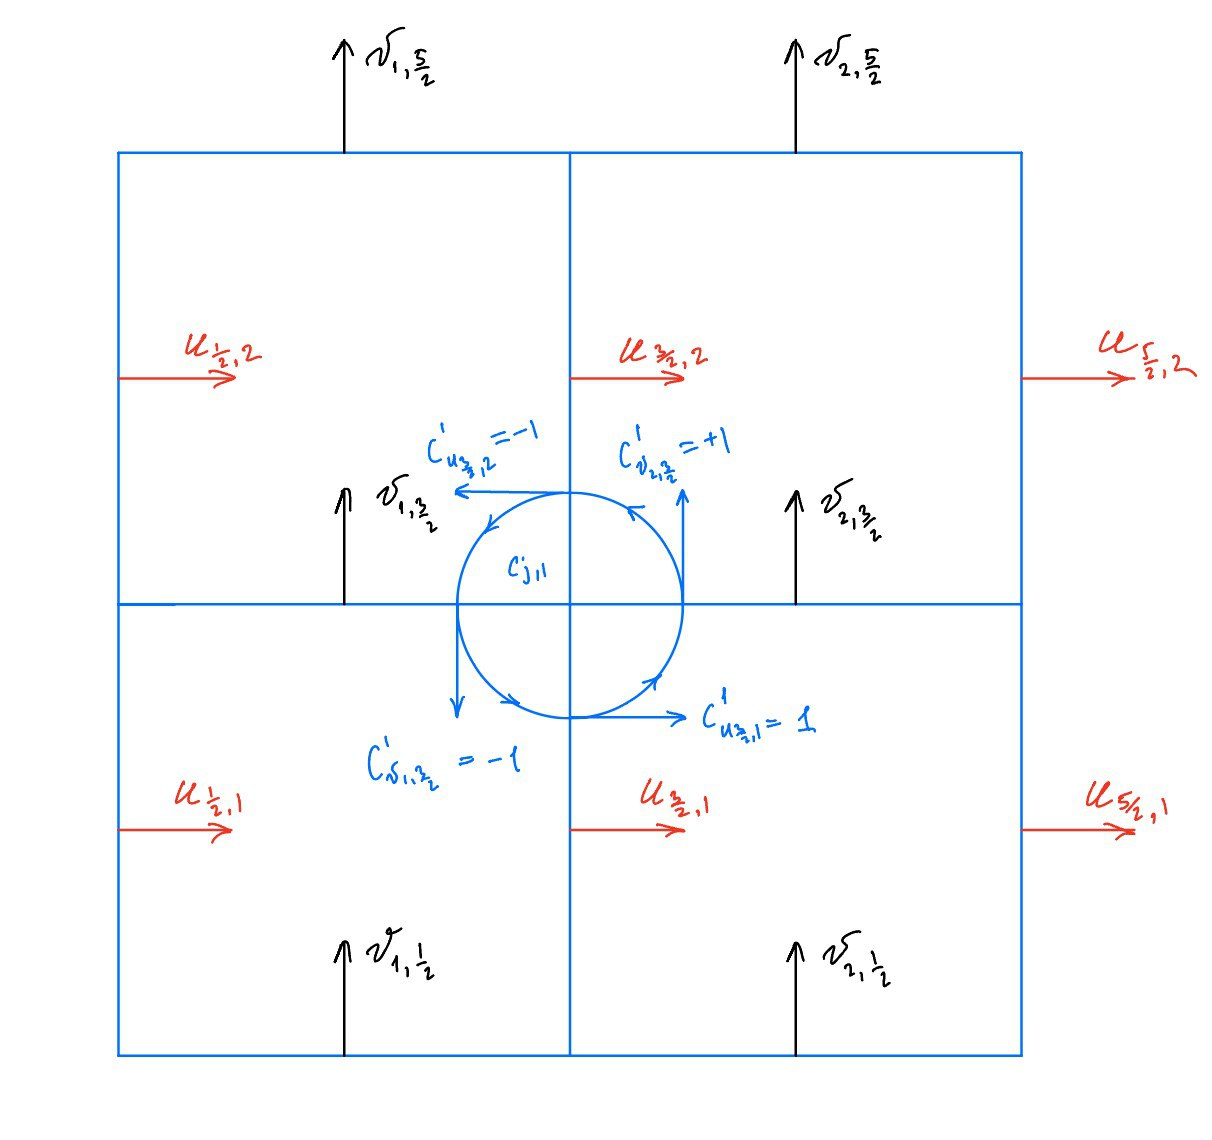
\includegraphics[width=0.40\paperwidth]{C-example-2x2}
  }
  \caption{$2\times 2$ example for $C$ matrix.}\label{fig:C-example-2x2}
\end{figure}
A more intuitive way of constructing the matrix $C$ relies on the utilization of counterclockwise vorticity around the nodes within the domain (\cref{fig:C-example-2x2}). If the direction of the velocity vector on the adjacent face aligns with the vorticity's direction, +1 is assigned to the corresponding row; conversely, -1 is assigned in the case of opposite directions of velocity and vorticity. After applying the above procedure we obtain
\begin{equation*}
  C = 
  \begin{bmatrix*}[r]
  1		\\
%  0		\\
  -1	\\
%  0		\\
  -1	\\
  1		\\
\end{bmatrix*}.
\end{equation*}

\begin{figure}[H]
\begin{center}
  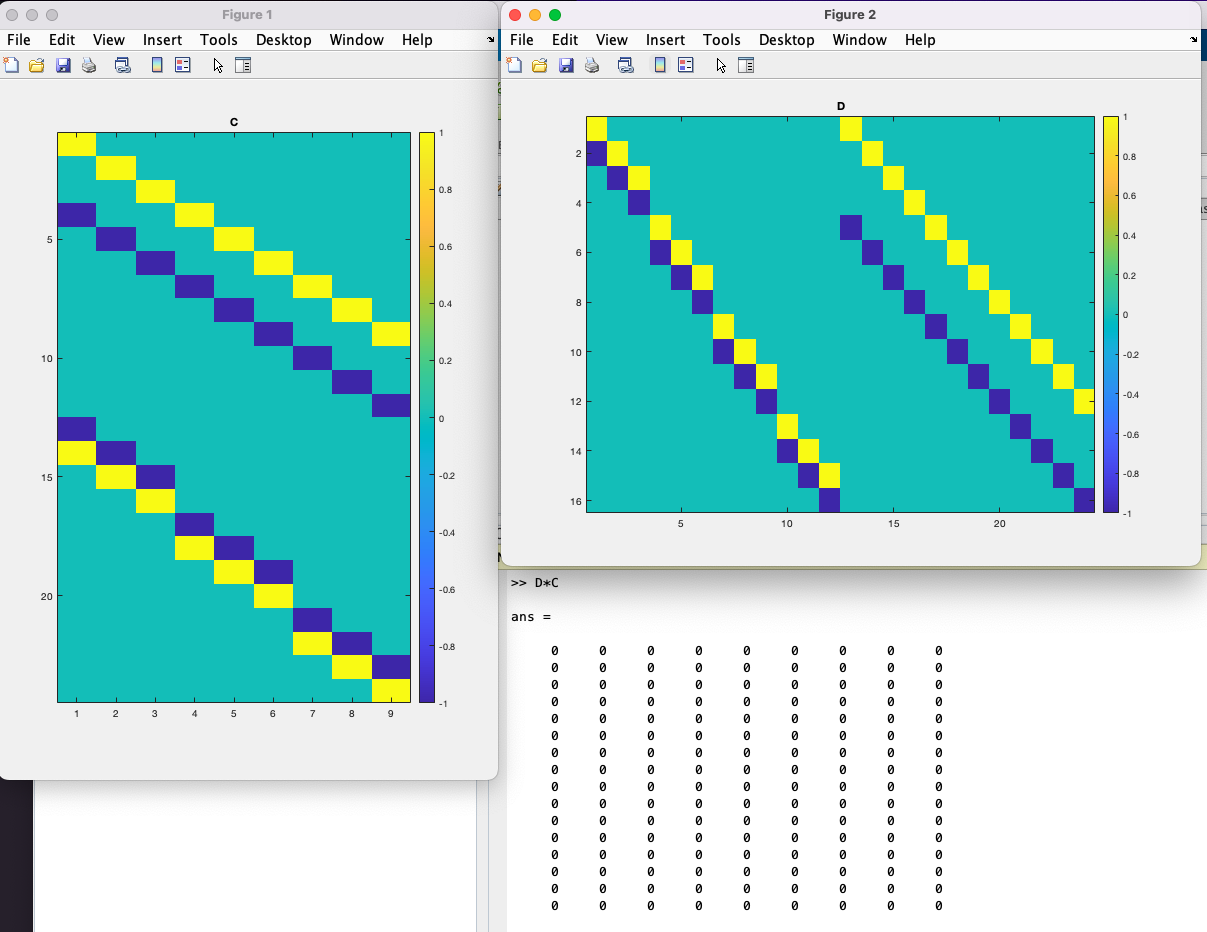
\includegraphics[width=0.75\textwidth]{Figures/D-C-DC}
\end{center}
\caption{Divergence and Curl matrices.}
\label{fig:DC}
\end{figure}
The matrix $C$ has dimensions corresponding to unknown velocities times the number of nodes around which these velocities revolve. 
	Figure~\ref{fig:DC} illustrates matrices $D$ and $C$ for a $4\times4$ grid with an open boundary on the right side of the domain. 
%Yellow squares represent $+1$ entries, while blue squares correspond to $-1$. 
The desired product then becomes $DC=0$. 
	$D=-G^T$ (from \cref{sec:discretization}) leads to important property $(DC)^T=C^TD^T=-C^TG=0$. 
	Premultiplying momentum equation in \cref{sys:discrete-nse} by $C^T$ creates $C^TGp=0$ term, which completely eliminates the pressure from our system.

In order to make use of efficient solvers, the matrix $C^TA$ can be made symmetric if multiplied by $C$ from the right. 
	We use the property of product $C^TC=-L$ being symmetric Laplacian and $C^TLC=-L^2$ being symmetric biharmonic operator with Dirichlet boundary conditions. 
	Matrix $C^TC=-L^2$ has zero boundary conditions for the vector it is applied to.
	Hence, the final chord of this method is the introduction of new variable called discrete streamfunction $\psi:q=C\psi$ as discussed at the beginning of this section.
	
	\cref{sys:discrete-nse} 
\begin{equation}
\left[\begin{array}{cc}
C^{\mathrm{T}} A C & C^{\mathrm{T}} E^{\mathrm{T}} \\
E C & 0
\end{array}\right]\left(\begin{array}{c}
\psi^{n+1} \\
\tilde{f}
\end{array}\right)=\left(\begin{array}{c}
C^{\mathrm{T}} r_1^n \\
\boldsymbol{v}_{\mathrm{B}}^{n+1}
\end{array}\right) .
\end{equation}

The left-hand side matrix is symmetric but in general indefinite, making a direct solution less efficient. The projection (fractional step) approach mimics Eqs. (9)-(11), and we obtain
\begin{equation}
  \begin{aligned}
& C^{\mathrm{T}} A C \psi^*=C^{\mathrm{T}} r_1^n, \\
& E C\left(C^{\mathrm{T}} A C\right)^{-1}(E C)^{\mathrm{T}} \tilde{f}=E C s^*-\boldsymbol{v}_{\mathrm{B}}^{n+1}, \\
& \psi^{n+1}=\psi^*-\left(C^{\mathrm{T}} A C\right)^{-1}(E C)^{\mathrm{T}} \tilde{f},
\end{aligned}
\end{equation}

	
\section{Fast method for uniform grid and simple boundary conditions}\label{sec:fast-method}

In this section we will show that a similar system to \cref{eqs:discrete-nse} can be solved using fast sine transforms, this method is, however, restricted to uniform grids. Mass matrix $M$ in this case becomes diagonal identity matrix. It is assumed that the values of the velocity are known in the region outside the computational domain, thus, we will apply simple Dirichlet BC's for normal and Neumann to tangential velocity components at the boundaries. Let us operate with $C^T$ on momentum equation from \cref{{eqs:discrete-nse}} in order to eliminate the pressure. We will obtain 
\begin{equation}
	\frac{\partial \gamma}{\partial t} + C^TE^T\tilde{f} = -\frac{1}{\operatorname{Re} \Delta ^2} C^TC\gamma + C^T \mathbf{N}(q)+ bc_{\gamma},
\end{equation}
where $\gamma=C^Tq$ is circulation, $\Delta$ stands for constant spacing in uniform grid and we used the fact that $Lq=-\frac{1}{\operatorname{Re}\Delta ^2} CC^Tq=-\frac{1}{\operatorname{Re}\Delta ^2} C\gamma$, since $Dq=0$. The last part is equivalent to $\nabla^2\boldsymbol{v}=\nabla(\nabla\cdot\boldsymbol{v})-\nabla\times\nabla\times\boldsymbol{v}=-\nabla\times\nabla\times\boldsymbol{v}$ taking into account continuity equation $\nabla\cdot\boldsymbol{v}=0$)

BC's we apply result in zero Dirichlet BC's for $\gamma$. The discrete Laplacian is diagonalized by a sine transform that is computed in $O(N \log_2 N)$ operations (here $N$ stands for the number of unknown $\gamma$ components). The sine transform pair is denoted as 
\begin{equation}
  \hat\gamma = S\gamma\leftrightarrow\gamma=S\hat\gamma,
\end{equation} 
where the operator $S$ is equal to inverse of itself due to the possible normalization process. For convenience the combination of fast sine transform with Laplace operator we denote 
\begin{equation}
  \Lambda = SC^TCS,
\end{equation}
which is a diagonal matrix with eigenvalues of $C^TC$ with integer coefficients. 

Using the same time marching procedure as in \cref{sec:discretization} we obtain 
%\begin{equation}
\begin{align}
& S\left(I+\frac{\beta \Delta t}{2} \Lambda\right) S \gamma^*=\left(I-\frac{\beta \Delta t}{2} C^{\mathrm{T}} C\right) \gamma^n +\frac{\Delta t}{2}\left(3 C^{\mathrm{T}} \mathbf{N}\left(q^n\right)-C^{\mathrm{T}} \mathbf{N}\left(q^{n-1}\right)\right)  +\Delta t b c_\gamma, \\
& E C\left(S \Lambda^{-1}\left(I+\frac{\beta \Delta t}{2} \Lambda\right)^{-1} S\right)(E C)^{\mathrm{T}} \tilde{f}=E C S \Lambda^{-1} S \gamma^*-\boldsymbol{v}_{\mathrm{B}}^{n+1},\label{eqn:modified-poisson} \\
& \gamma^{n+1}=\gamma^*-S\left(I+\frac{\beta \Delta t}{2} \Lambda\right)^{-1} S(E C)^{\mathrm{T}} \bar{f}.
\end{align}
%\end{equation}
We can obtain vector $\boldsymbol{v}$ for all previous time steps using
\begin{equation}
	q^n=C\psi^n + bc_q, \psi^n=S\Lambda^{-1}S\gamma^n + bc_\psi.
\end{equation}

In the new system of equations only one linear system (\cref{eqn:modified-poisson}) needs to be solved. This linear system has positive definite left-hand side operator. This system requires 
\begin{equation}
	O(N(2\log_2 N + N_{bw} + 4d))
\end{equation}
against
\begin{equation}
	O(N(N_{bw} + (2d+1)j + 4d))
\end{equation}
in step 2 of \cref{algorithm:projection}, where $N_{bw}$ is the bandwidth of the body-force regularization or interpolation operators, $d$ is the dimension of the problem (2 or 3 dimensions) and $j$ is the order of approximate Taylor-series inverse of matrix $A$. The speedup for $128\times128$ grid  in 2D is about 10, and 30 for $128\times128\times128$ in 3D. It should be mentioned that there is no iterative error in solving the equation, only round-off error remains. In the case of stationery body the Poisson-alike equation for body forces can be efficiently solved using Cholesky decomposition. 

In conclusion of this section it is required to say that this fast method can only be applied to simple boundary conditions, which take only a small portion of all possible scenarios. Nevertheless, in the next section we will discuss the workaround for implementing boundary conditions with a small trade-off.

\section{Multi-domain approach}\label{sec:multi-domain-approach}

The fast sine transform method relies on simple boundary conditions (Dirichlet for normal and Neumann for tangential velocities at the boundary). Stating this for the small domain will result in two sources of errors
\begin{enumerate}
  \item Extensive, algebraically decaying potential flow induced by the body.
  \item Vorticity may advect or diffuse through the boundary. 
\end{enumerate}
These errors are minimized by using a large non-uniform domain as well as using convective boundary conditions discussed in \cref{sec:discretization} which are incompatible with fast sine method in \cref{sec:fast-method}. In this section we present the way of keeping these error minimizing strategies as well as applying fast sine method together. 

The basic idea is to consider nested domains as in \cref{fig:multi-domain}. The circulation $\gamma$ on the inner mesh is interpolated onto the coarser (larger) mesh couple of times, then the Poisson equation is solved on the outer domain. This solution is then interpolated along the boundary of the inner mesh and the Poisson equation is solved with the "corrected" boundary values on smaller meshes.  This technique is used recursively a number of times. The domain coarsening factor is 2 at each grid level. 

\begin{figure}[H] % here - h, bottom - b, top - t
  \centering{
  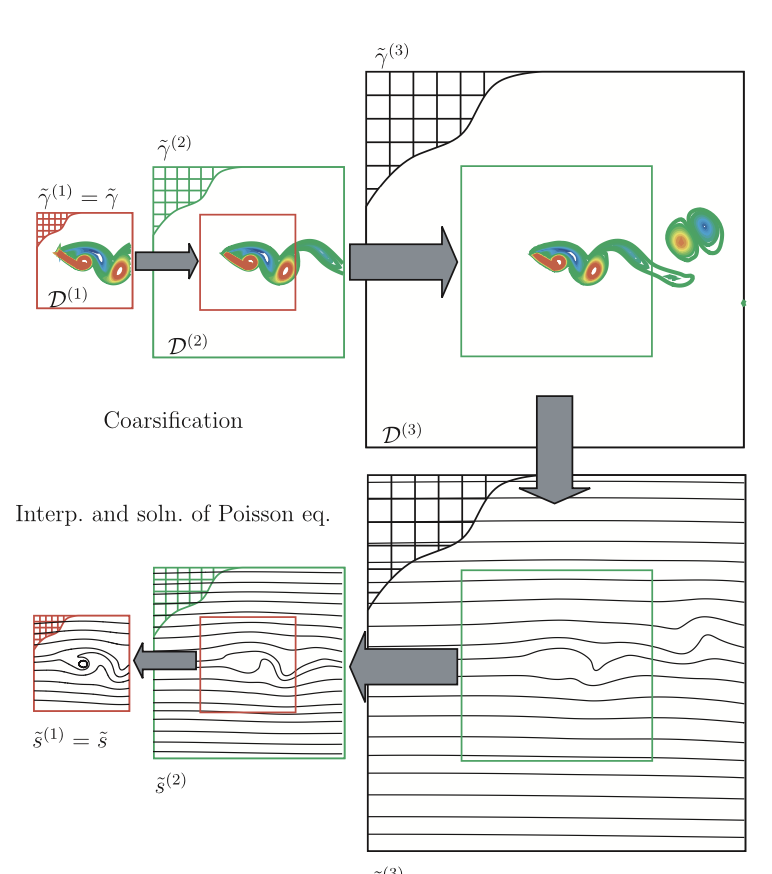
\includegraphics[width=0.40\paperwidth]{fig4}
  }
  \caption{Three layer multi-domain.}\label{fig:multi-domain}
\end{figure}


The method is described as follows. Let us defined the domain of each grid as $\mathscrsfs{D}^{(k)}$, $k=1,2,3,\dots,N_g$, where $k=1$ and $k=N_g$ stand for the smallest and largest domains respectively. We then define a multi-domain inverse Laplacian
\begin{equation}
	\tilde\psi=S\overline{\Lambda^{-1}}S\tilde\gamma,
\end{equation}
where $\tilde\gamma$ is an arbitrary input vector, $\tilde\psi$ is streamfunction solution, and the operator $S\overline{\Lambda^{-1}}S$ implies the following operations:
\begin{align}
	&\tilde\gamma^{(1)}=\tilde\gamma\\
	&\tilde\gamma^{(k)}=
		\begin{cases}
			\tilde\gamma^{(k)} \text{ for } x\in \mathscrsfs{D}^{(k)}\backslash\mathscrsfs{D}^{(k-1)},\\
			P^{(k-1)\to(k)}(\tilde\gamma^{(k-1)}) \text{ for } x\in\mathscrsfs{D}^{(k-1)},\\
			\qquad k=2,3,\dots,N_g,
		\end{cases}\\
	&\tilde\psi^{(N_g+1)}=0,\\
	&\tilde\psi^{(k)}=S\Lambda^{-1}S\tilde\gamma^{(k)} + bc_\psi\left[P^{(k+1)\to(k)}(\tilde\psi^{(k+1)}) \right], k=N_g,N_g-1,\dots,1,\\
	&\tilde\psi = S\overline{\Lambda^{-1}}S\tilde\gamma=\tilde\psi^{(1)}.
\end{align}
In the process above $P^{(k-1)\to(k)}$ and $P^{(k+1)\to(k)}$ are fine-to-coarse and coarse-to-fine interpolation operators. In 2D case the fine-to-coarse interpolation uses 9-point stencil, that is
\begin{equation}\label{eqn:fine-to-coarse}
\begin{aligned}
	P^{(k-1) \rightarrow(k)}\left(\tilde{\gamma}^{(k-1)}\right)_{2 i, 2 j}= 
	& \tilde{\gamma}_{i, j}^{(k-1)}+\frac{1}{2} \tilde{\gamma}_{i-1, j}^{(k-1)}+\frac{1}{2} \tilde{\gamma}_{i+1, j}^{(k-1)} +\frac{1}{2} \tilde{\gamma}_{i, j-1}^{(k-1)}+\frac{1}{2} \tilde{\gamma}_{i, j+1}^{(k-1)}+\\
	&+\frac{1}{4} \tilde{\gamma}_{i-1, j-1}^{(k-1)} +\frac{1}{4} \tilde{\gamma}_{i+1, j-1}^{(k-1)}+\frac{1}{4} \tilde{\gamma}_{i-1, j+1}^{(k-1)}  +\frac{1}{4} \tilde{\gamma}_{i+1, j+1}^{(k-1)}.
\end{aligned}
\end{equation}
The coefficients in \cref{eqn:fine-to-coarse} add up to 4, since the circulation $\tilde\gamma$  is the vorticity multiplied by the area and coarsification of the grid by factor of two leads to increase in a factor of 4 increase in cell area. The reverse coarse-to-fine interpolation is performed linearly in case of a mid-point and by taking the value from the coarser mesh if points coincide, note, that this only has to be performed along the boundary of the finer mesh (i.e. four straight segments). 
Using the multi-domain approach for circulation and solving the Poisson equation, we can finally write the system of equations to be solved for each time step. 
\begin{equation}
\begin{aligned}
&\begin{aligned}
& S\left(I+\frac{\beta \Delta t}{2} \Lambda\right) S \gamma^{(k)^*} \\
& =\left(I-\frac{\beta \Delta t}{2} C^{\mathrm{T}} C\right) \gamma^{(k)^n}+\frac{\Delta t}{2}\left(3 C^{\mathrm{T}} \mathscr{N}\left(q^{(k)^n}\right)-C^{\mathrm{T}} \mathscr{N}\left(q^{(k)^{n-1}}\right)\right) \\
& \quad+\frac{\Delta t}{2} b c_\gamma\left(\left[P^{(k+1) \rightarrow(k)}\left(\gamma^{(k+1)^*}\right)\right]+\left[P^{(k+1) \rightarrow(k)}\left(\gamma^{(k+1)^n}\right)\right]\right) \\
& \quad k=N_g, N_{g-1}, \ldots, 1, \\
& E C\left(S \overline{\Lambda^{-1}}\left(I+\frac{\beta \Delta t}{2} \Lambda\right)^{-1} S\right)(E C)^{\mathrm{T}} \tilde{f}=E C S \overline{\Lambda^{-1}} S \gamma^{(1)^*}-\boldsymbol{v}_{\mathrm{B}}^{n+1},
\end{aligned}\\
&\gamma^{n+1}=\gamma^{(1)^*}-S\left(I+\frac{\beta \Delta t}{2} \Lambda\right)^{-1} S(E C)^{\mathrm{T}} \tilde{f}\\
&\psi^{n+1}=S \overline{\Lambda^{-1}} S \gamma^{n+1} .
\end{aligned}
\end{equation}

When the vorticity crosses the boundary of a grid level, $\gamma^{(j)}$ fields are not smooth across the interfaces, especially at the coarsest levels. Results show the propagation of a vortex through mesh levels and slight reflections of the circulation near the boundary, however, the errors remain confined to a small region near the boundary and diffused over time by the physical viscosity. 



	
\section{Summary}\label{sec:summary}
	

\pagebreak
\bibliographystyle{plain}
\bibliography{Zotero.bib}
 

\pagebreak
\appendix
\section{Appendix}

\subsection{Transient schemes}

\end{document}
